%%%%%%%%%%%%%%%%%%%%%%%%%%%%%%%%%%%%%%%%%%%%%%%%%%%%%%%%%%%%%%%%%%%%%%%%
% Preamble
%%%%%%%%%%%%%%%%%%%%%%%%%%%%%%%%%%%%%%%%%%%%%%%%%%%%%%%%%%%%%%%%%%%%%%%%
\documentclass[11pt]{article}
%
% Packages and other includes
% Pagination
\usepackage[letterpaper, margin=1.25in]{geometry}
%
% Fonts
\usepackage[T1]{fontenc} % best for Western European languages
\usepackage{lmodern} % Latin Modern instead of CM
\usepackage{textcomp} % required to get special symbols
%
% Math
\usepackage{amsmath, amssymb}
\usepackage{braket}
%
% Graphics, floats, tables
\usepackage{graphicx, xcolor, float, array}
\usepackage{subcaption}
%
% Hyperlinks
\usepackage{hyperref}
%
% Bibliography
\usepackage[style=numeric, sorting=none, backend=biber]{biblatex}
\addbibresource{references.bib}
%
% Revision (see Makefile)
%\input{revision.tex}
%
% Definitions and settings
% Paragraph indent and spacing
\setlength{\parskip}{0.4\baselineskip}
\setlength{\parindent}{0in}
%
% Math mode version of "r" column type (requires array package)
\newcolumntype{R}{>{$}r<{$}}
%
%comments
\newcommand{\brian}[1]{{\color{orange} #1}}
% Title, authors, date
\title{\textbf{Is Using TPSS and TPSSh for RPA better for noncovalent
    calculations?}}
\author{Thanh Huynh and Brian Nguyen}
\date{11/27/2020 -- 01/10/2021 }
%
%
%%%%%%%%%%%%%%%%%%%%%%%%%%%%%%%%%%%%%%%%%%%%%%%%%%%%%%%%%%%%%%%%%%%%%%%%
% Main document
%%%%%%%%%%%%%%%%%%%%%%%%%%%%%%%%%%%%%%%%%%%%%%%%%%%%%%%%%%%%%%%%%%%%%%%%
%

\begin{document}

\maketitle

\section{Introduction}

A potent cytotoxin, called chlorolissoclimide, was discovered
in the sea squirt and could potentially be useful in cancer therapeutics
or other pharmaceuticals, such as medication for COVID-19. This chemical
induces cell death by obstructing production of proteins. An interesting
ribosome-drug interaction was revealed to form a halogen-pi bond however,
characteristics of the bond are still unknown. Halogen bonds are formed
when a halogen interacts with other atoms within a molecule.Researching
this specific interaction could help with creating new cancer therapeutic
or improving medication.

Following up the previous report, random phase approximation (RPA) was
chosen to be used with different functionals. The TPSS and TPSSh
functionals may describe the halogen-pi bond more accurately than PBE.
To investigate which functional performs better, the X40 test set serves
as a benchmark for TPSS, TPSSh, and PBE calculations.  


\section{Methods}

Based on the previous report, the 3-4 extrapolation of the RIRPA
correlation energy was a good balance between efficiency and accuracy.
The X40 Test Set was used to benchmark the method's accuracy for 
noncovalent interactions involving halogens. The test set contains 40
complexes with despersion, induction, dipole-dipole, stack, hydrogen
bond, halogen bond, and halogen-pi bond interations.

To conserve time, a set of eight complexes from the X40 test set were
chosen based on error from the previous report to study basis set
convergences. Calculations were computed with basis sets def2-QZVP,
cc-pVTZ, and cc-pVQZ. The RPA energies were computed based on converged
orbitals from TPSS and TPSSh and resolution of identity (RI) was included
to improve efficiency. The Hartree Exact Exchange (HXX) total energy and
RIRPA correlation energy were recorded from the supermolecule and
monomers of each complex to compute interaction energies. The interaction
energies from the selected complexes were extrapolated using the
supramolecular approach. Due to the basis set superposition error (BSSE),
counterpoise corrections (CP) were applied to the RIRPA correlation
energy as well.

\section{Results}

\begin{figure}[H]
  \centering
  \begin{subfigure}{\textwidth}
    \center
    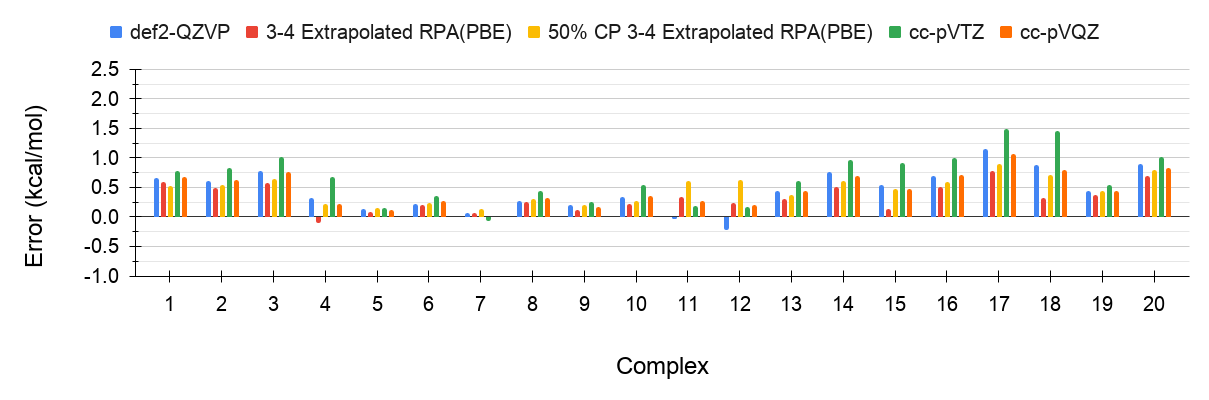
\includegraphics[scale=0.35]{def2-QZVP_1.png}
    \label{fig:def2-QZVP_1}
  \end{subfigure}
  \begin{subfigure}{\textwidth}
    \center
    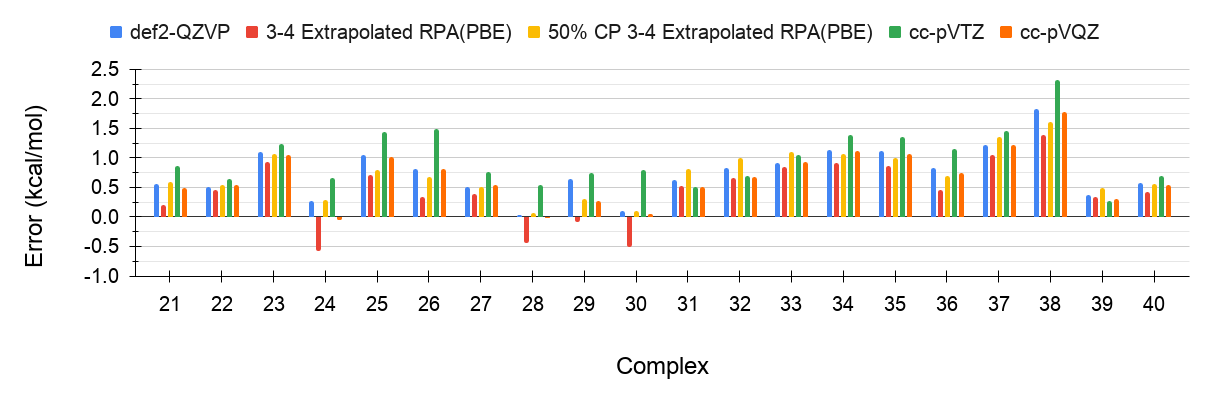
\includegraphics[scale=0.35]{def2-QZVP_2.png}
    \label{fig:def2-QZVP_2}
  \end{subfigure}
  \caption{The binding energy errors (kcal/mol) for X40 test set computed
    for RPA(PBE) methods with basis functions def2-QZVP, cc-pVTZ, and
    cc-pVQZ. Negative sign indicates overbinding.}
  \label{fig:def2-QZVP Error}
\end{figure}

For most complexes, the method using the def2-QZVP basis function yields
an error greater than the 3-4 extrapolated, 50 percent CP
extrapolated, and cc-pVQZ. 

\begin{table}[hbpt]
  \caption{Statistical analysis of def2-QZVP, 3-4 Extrapolation, 50 3-4
    Extrapolation, cc-pVTZ, and cc-pVQZ for the X40 test set. The mean
    relative error (kcal/mol), mean absolute error (kcal/mol), and
    standard deviation (kcal/mol). Negative sign indicates overbinding.}
  \centering
  \begin{tabular}{c|c|c|c|c|c}
    & def2-QZVP & 3-4 Extrapolation & 50 3-4 Extrapolation & cc-pVTZ  &
    cc-pVQZ \\
    \hline\hline
    Mean Error & 0.6031 & 0.3895 & 0.5981 & 0.8334 & 0.5768 \\
    Mean Abs Error & 0.6161 & 0.4744 & 0.5980 & 0.8372 & 0.5807 \\
    Standard Deviation & 0.4122 & 0.4044 & 0.3495 & 0.4783 & 0.3934 \\
  \end{tabular}
  \label{tab:table_1}
\end{table}

\begin{figure}[H]
  \centering
  \begin{subfigure}{.5\textwidth}
    \centering
    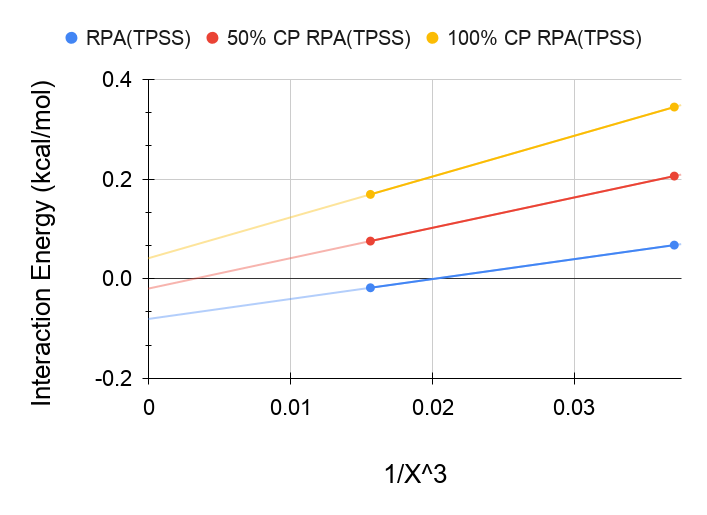
\includegraphics[scale=0.3]{tpss-1.png}
    \caption{RPA(TPSS)}
    \label{fig:tpss_1}
  \end{subfigure}%
  \begin{subfigure}{.5\textwidth}
    \centering
    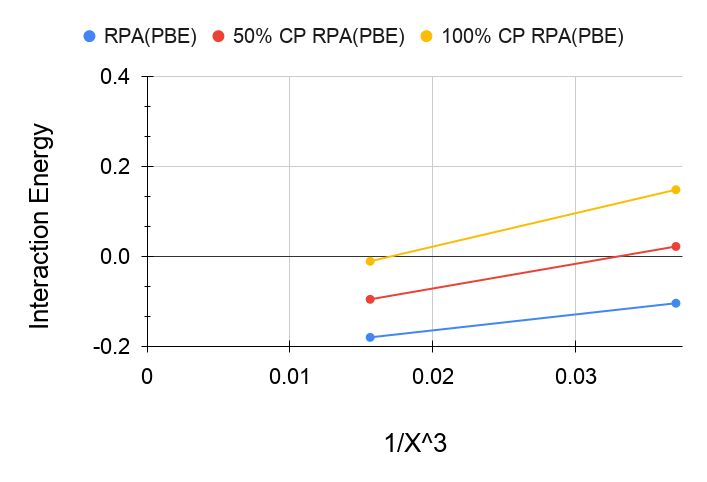
\includegraphics[scale=0.3]{tpssh-1.png}
    \caption{RPA(TPSSh)}
    \label{fig:tpssh_1}
  \end{subfigure}
  \caption{Basis sets convergence plot for RPA(TPSS) and RPA(TPSSh) is
    presented for complex 1. Dunning's basis sets were used for all atoms
    and 1/X$^3$, where X is the cardinal number, was used for
    extrapolation to form linear lines. Complex 1 contains dispersion
    interaction with fluorine.}
  \label{fig:complex_1}
\end{figure}

The convergence plot for RPA(TPSS) and RPA(TPSSh) both don't appear to be
converging since the extrapolated lines are nearly parallel. The plot for
RPA(TPSSh) also approaches a value that is more negative than RPA(TPSS).


\begin{figure}[H]
  \centering
  \begin{subfigure}{.5\textwidth}
    \centering
    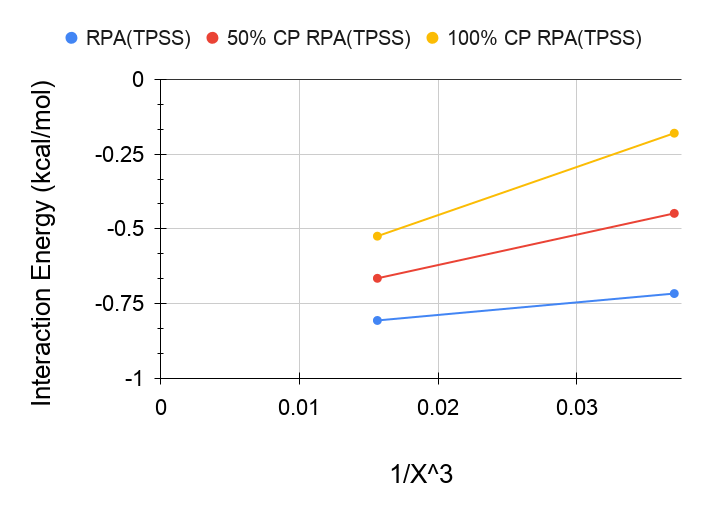
\includegraphics[scale=0.3]{tpss-8.png}
    \caption{RPA(TPSS)}
    \label{fig:tpss_8}
  \end{subfigure}%
  \begin{subfigure}{.5\textwidth}
    \centering
    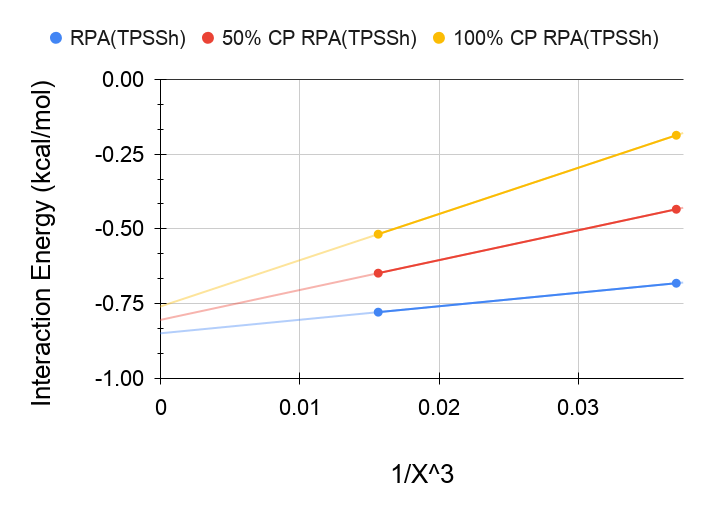
\includegraphics[scale=0.3]{tpssh-8.png}
    \caption{RPA(TPSSh)}
    \label{fig:tpssh_8}
  \end{subfigure}
  \caption{Basis sets convergence plot for RPA(TPSS) and RPA(TPSSh) is
    presented for complex 8. Dunning's basis sets were used for all atoms
    and 1/X$^3$, where X is the cardinal number, was used for extrapolation
    to form linear lines. Complex 8 contains induction interactions with
    chlorine.}
  \label{fig:complex_8}
\end{figure}

The convergence plots for RPA(TPSS) and RPA(TPSSh) do not appear to
converge. The 50 percent CP and 100 percent CP lines are nearly parallel.


\begin{figure}[H]
  \centering
  \begin{subfigure}{.5\textwidth}
    \centering
    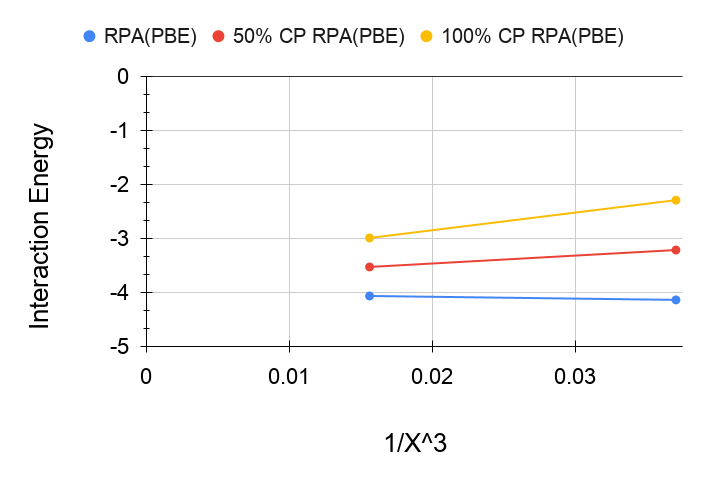
\includegraphics[scale=0.3]{tpss-11.png}
    \caption{RPA(TPSS)}
    \label{fig:tpss11}
  \end{subfigure}%
  \begin{subfigure}{.5\textwidth}
    \centering
    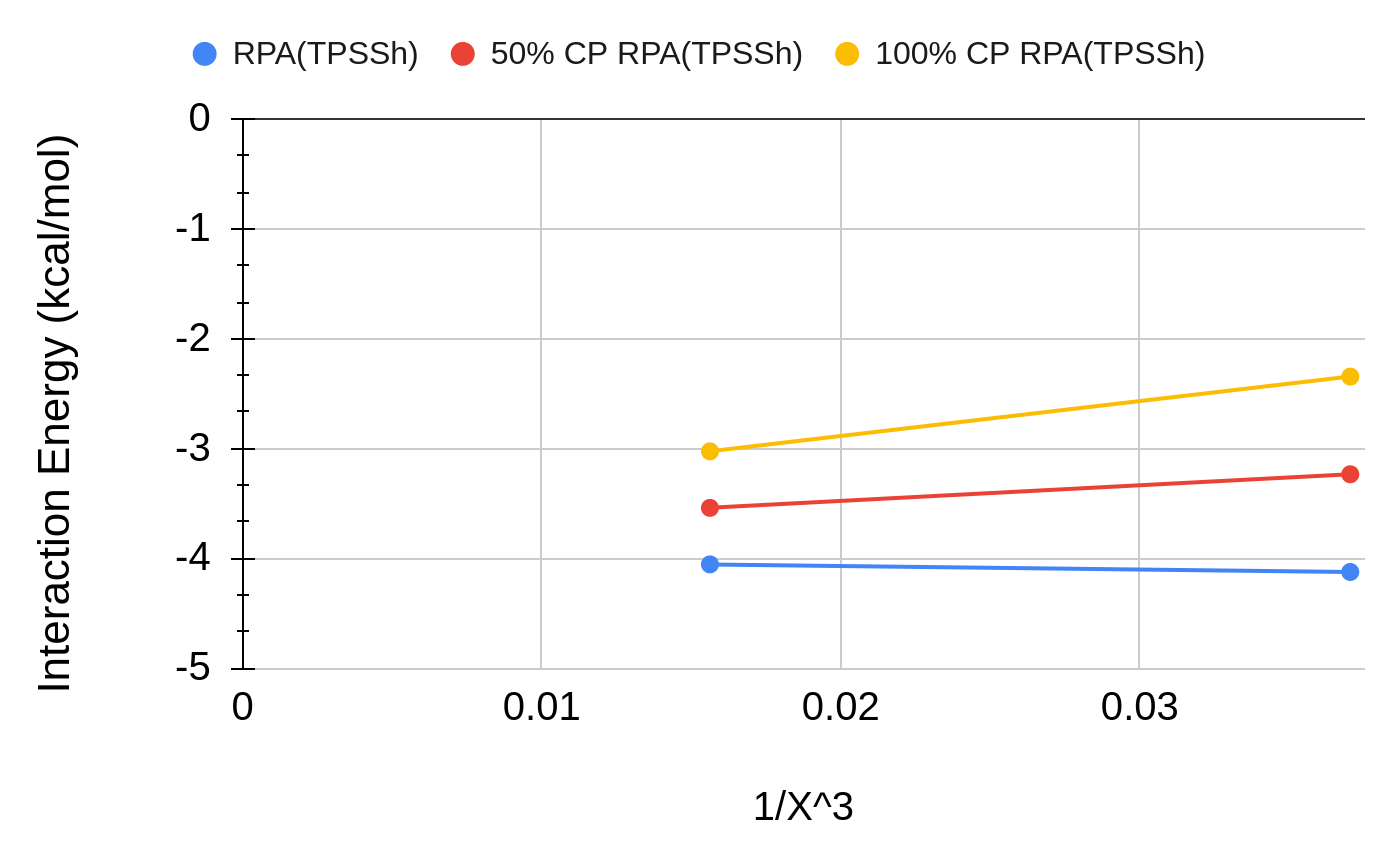
\includegraphics[scale=0.3]{tpssh-11.png}
    \caption{RPA(TPSSh)}
    \label{fig:tpssh_11}
  \end{subfigure}
  \caption{Basis sets convergence plot for RPA(TPSS) and RPA(TPSSh) is
    presented for complex 11. Dunning's basis sets were used for all
    atoms and 1/X3, where X is the cardinal number, was used for
    extrapolation to form linear lines. Complex 11 contains stack
    interactions with fluorine.}
  \label{fig:complex_11}
\end{figure}

Both the RPA(TPSS) and RPA(TPSSh) plots for complex 11 are converging
to one value as they approach 0. The interaction energy for RPA(TPSS)
appears to be negative while the energy for RPA(TPSSh) is positive.


\begin{figure}[H]
  \centering
  \begin{subfigure}{.5\textwidth}
    \centering
    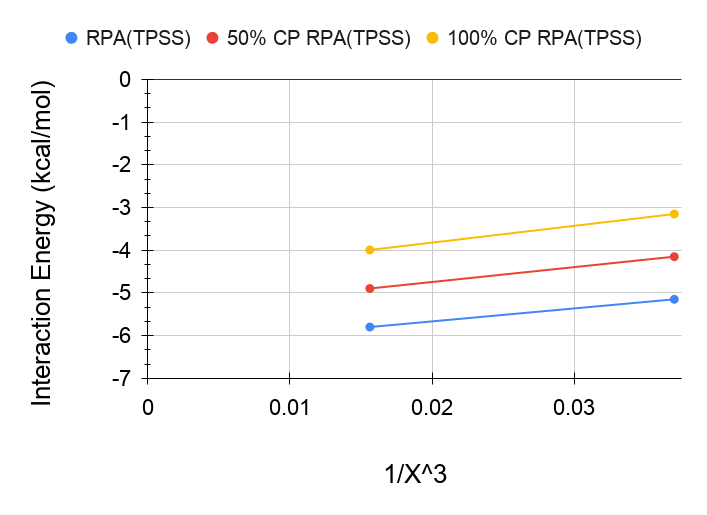
\includegraphics[scale=0.3]{tpss-24.png}
    \caption{RPA(TPSS)}
    \label{fig:tpss_24}
  \end{subfigure}%
  \begin{subfigure}{.5\textwidth}
    \centering
    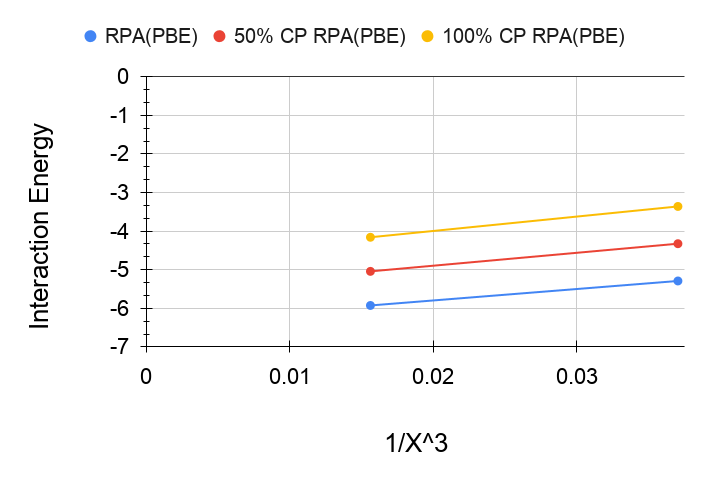
\includegraphics[scale=0.3]{tpssh-24.png}
    \caption{RPA(TPSSh)}
    \label{fig:tpssh_24}
  \end{subfigure}
  \caption{Basis sets convergence plot for RPA(TPSS) and RPA(TPSSh) is
    presented for complex 24. Dunning's basis sets were used for all
    atoms and 1/X3, where X is the cardinal number, was used for
    extrapolation to form linear lines. Complex 24 contains halogen 
    bonding with iodine.}
  \label{fig:complex_24}
\end{figure}

For complex 24, both RPA(TPSS) and RPA(TPSSh) do not converge at all.
The lines for both plots are parallel to each other as they approach 0.


\begin{figure}[H]
  \centering
  \begin{subfigure}{.5\textwidth}
    \centering
    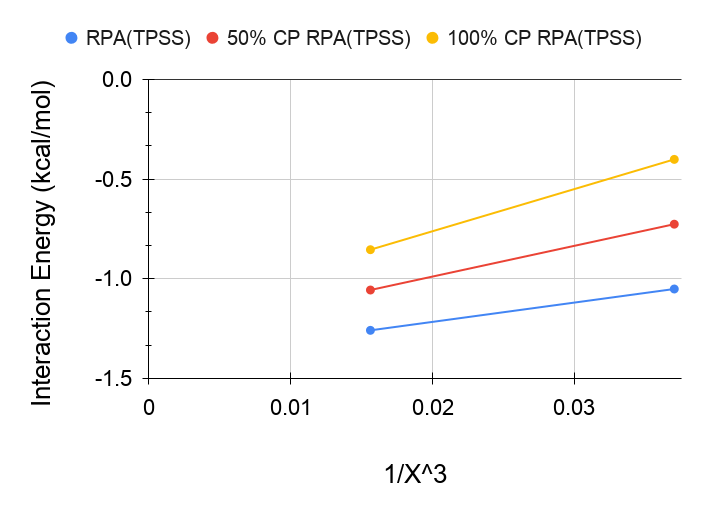
\includegraphics[scale=0.3]{tpss-27.png}
    \caption{RPA(TPSS)}
    \label{fig:tpss_27}
  \end{subfigure}%
  \begin{subfigure}{.5\textwidth}
    \centering
    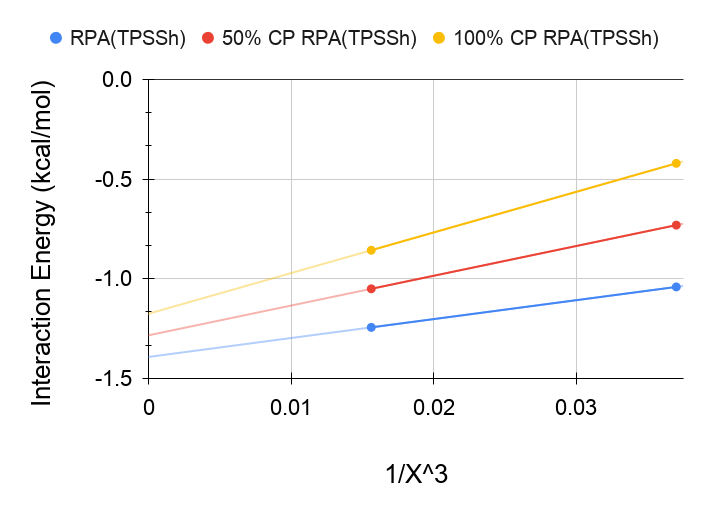
\includegraphics[scale=0.3]{tpssh-27.png}
    \caption{RPA(TPSSh)}
    \label{fig:tpssh_27}
  \end{subfigure}
  \caption{Basis sets convergence plot for RPA(TPSS) and RPA(TPSSh) is
    presented for complex 27. Dunning's basis sets were used for all
    atoms and 1/X3, where X is the cardinal number, was used for
    extrapolation to form linear lines. Complex 27 contains halogen-pi
    bonding with bromine.}
  \label{fig:complex_27}
\end{figure}

The RPA(TPSS) and RPA(TPSSh) convergence plots look similar and both don't
converge to one point. The extrapolated lines from cc-pVTZ to cc-pVQZ
appear nearly parallel with each other.

\begin{figure}[H]
  \centering
  \begin{subfigure}{.5\textwidth}
    \centering
    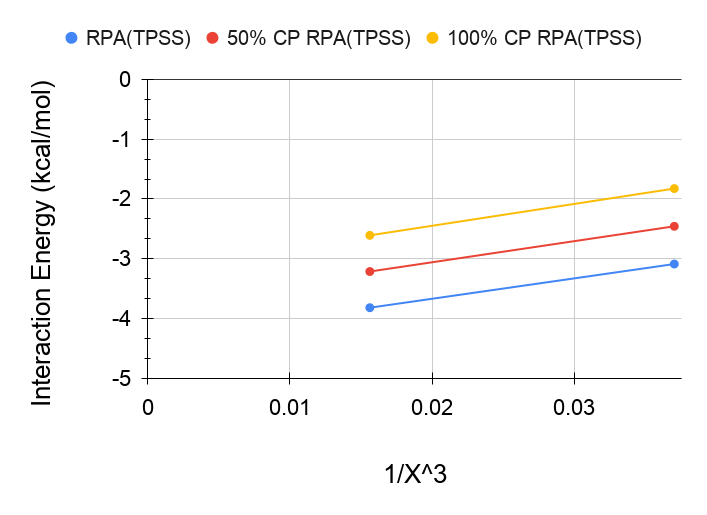
\includegraphics[scale=0.3]{tpss-30.png}
    \caption{RPA(TPSS)}
    \label{fig:tpss_30}
  \end{subfigure}%
  \begin{subfigure}{.5\textwidth}
    \centering
    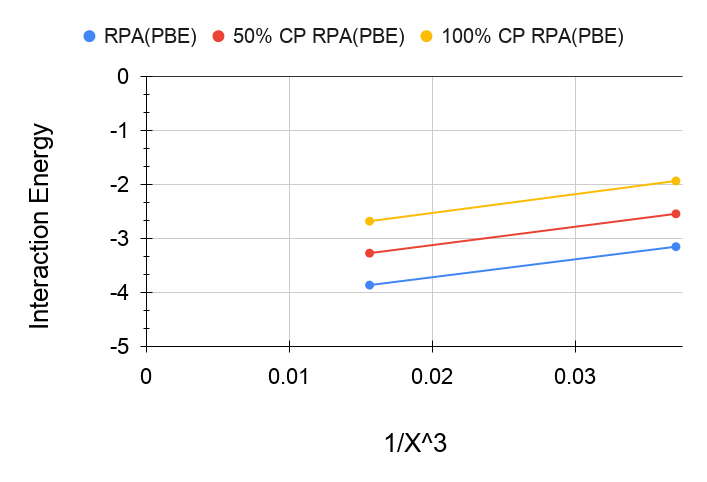
\includegraphics[scale=0.3]{tpssh-30.png}
    \caption{RPA(TPSSh)}
    \label{fig:tpssh_30}
  \end{subfigure}
  \caption{Basis sets convergence plot for RPA(TPSS) and RPA(TPSSh) is
    presented for complex 30. Dunning's basis sets were used for all
    atoms and 1/X3, where X is the cardinal number, was used for
    extrapolation to form linear lines. Complex 30 contains halogen-pi
    bonding with iodine.}
  \label{fig:complex_30}
\end{figure}

The convergence plot for RPA(TPSS) and RPA(TPSSh) both do not converge
as the extrapolated lines approach 0. The lines for RPA, 50 percent CP,
and 100 percent CP appear to be parallel.

\begin{figure}[H]
  \centering
  \begin{subfigure}{.5\textwidth}
    \centering
    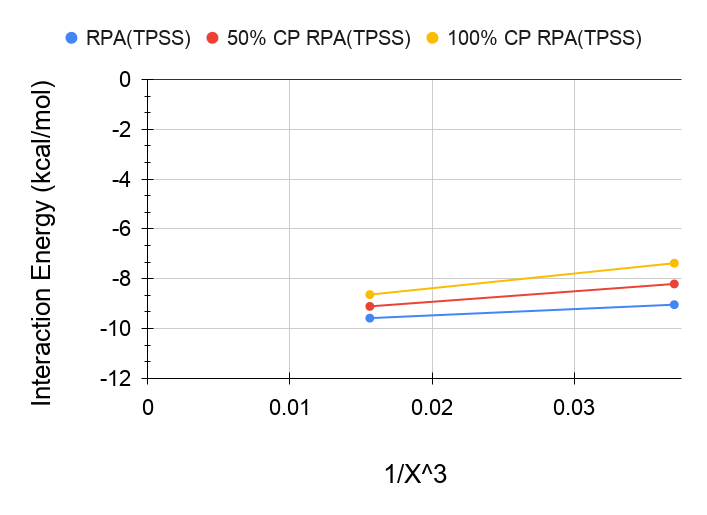
\includegraphics[scale=0.3]{tpss-38.png}
    \caption{RPA(TPSS)}
    \label{fig:tpss_38}
  \end{subfigure}%
  \begin{subfigure}{.5\textwidth}
    \centering
    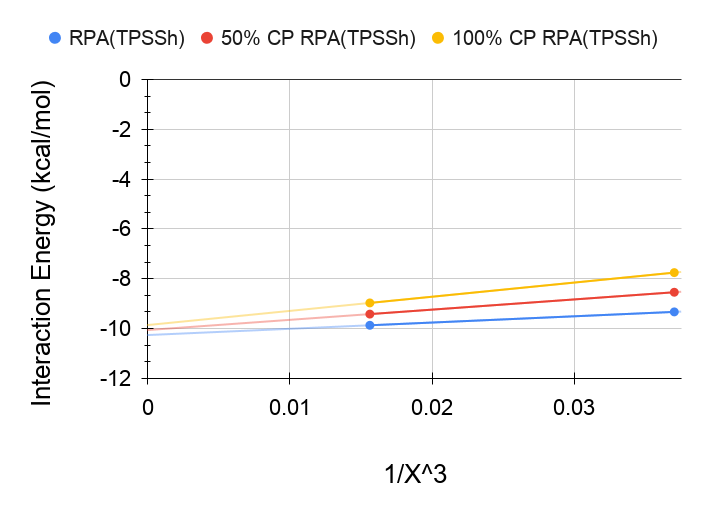
\includegraphics[scale=0.3]{tpssh-38.png}
    \caption{RPA(TPSSh)}
    \label{fig:tpssh_38}
  \end{subfigure}
  \caption{Basis sets convergence plot for RPA(TPSS) and RPA(TPSSh) is
    presented for complex 38. Dunning's basis sets were used for all
    atoms and 1/X3, where X is the cardinal number, was used for
    extrapolation to form linear lines. Complex 38 contains hydrogen
    bonding with chlorine.}
  \label{fig:complex_38}
\end{figure}

The convergence plots both don't converge as the lines approach 0. The
extrapolated line from cc-pVTZ to cc-pVQZ for RPA and 50 percent CP
appear to be parallel for the RPA(TPSS) and RPA(TPSSh) plots.

\brian{yada yada see Fig. \ref{fig:<name>}}




\section{Conclusions}

After investigating the binding energy errors for the X40 test set,
def2-QZVP is revealed to be a good balance between accuracy and
efficiency. The mean error of def2-QZVP,0.603 kcal/mol, is between the
mean error of cc-pVTZ, 0.833 kcal/mol, and cc-pVQZ, 0.576 kcal/mol.
def2-QZVP yields good results compared to cc-pVTZ and cc-pVQZ since it
does not have any CP to correct BSSE.

Using TPSS and TPSSh functionals for RPA do not describe the different
interactions better than PBE. The seven complexes chosen based on error
don't show any improvements because complexes 1, 8, 24, 27, 30, and 38
did not converge. When compared to the results from the previous report,
the error of the 3-4 extrapolation of RPA(TPSS) and RPA(TPSSh) were
greater than the error of RPA(PBE). It is still recommended to use
RPA(PBE) for noncovalent calculations.


\printbibliography

\end{document}
